\title{Continuum Stewart-Gough Teleoperation}
\author{John Till}
\date{}

\documentclass[12pt]{article}

\usepackage[a4paper, margin=0.75in]{geometry}
\usepackage[colorlinks=true,urlcolor=blue]{hyperref}
\usepackage{amsmath,amssymb}
\usepackage{graphicx}

\usepackage{xcolor}
\definecolor{OffWhite}{rgb}{0.93,0.93,0.93}
\definecolor{QtCommentColor}{rgb}{0,0.5,0}
\definecolor{QtKeywordColor}{rgb}{0.5,0.5,0}
\definecolor{QtPurpleColor}{rgb}{0.5,0,0.5}
\definecolor{QtGlobal}{rgb}{0.808,0.361,0}
\definecolor{QtFunctionColor}{rgb}{0,0.404,0.486}

\usepackage[T1]{fontenc} %for upquotes in listings
\usepackage{textcomp} %for upquotes in listings
\usepackage{listings}
\lstset{
		language=C++,
		escapeinside={!-}{-!},
		upquote=true,
		%
		otherkeywords={Vector3d, DiagonalMatrix, VectorXd, Matrix3d, Map, MatrixXd, Vector6d, Vector2d,
									std, QtCharts, QChart, QLineSeries, MainWindow, QKeyEvent, QPen, QColor,
									QList, QPointF, Matrix3Xd, Horizontal, Vertical,
									waitOnWorkers, setWorkerState, integrateRod, setJacobianOfLeg,
									UnitX, pow, transpose, segment, UnitZ, cross, hat_postmultiply,
									Zero, Identity, UnitY, cosseratRodOde, ode4, cols, row, main, shootingFunction,
									block, linear_rotation_error, solveLevenbergMarquardt, plot, Ones, join,
									Ry, Rz, initialize_StewartGough_pattern, clock, endl, jacobianFunction, workerFunction,
									sin, cos, finished, inverseKinematicsCSG, initializeCharts, refreshCharts,
									keyPressEvent, resetKinematicsSolver, setTitleText, addWidget, fromRgb, setWidthF,
									setPen, addSeries, createDefaultAxes, legend, hide, axes, back, setRange,
									getLegCenterline, replace, first, hat, resetCSG, last,
									Key_Q, Key_W, Key_E, Key_A, Key_S, Key_D, Key_U, Key_I, Key_O,
									Key_J, Key_K, Key_L},
    morekeywords=[2]{Vector3d, DiagonalMatrix, VectorXd, Matrix3d, Map, MatrixXd, Vector6d, Vector2d,
		                 std, QtCharts, QChart, QLineSeries, MainWindow, QKeyEvent, QPen, QColor,
										 QList, QPointF, Matrix3Xd, Horizontal, Vertical,
										 Key_Q, Key_W, Key_E, Key_A, Key_S, Key_D, Key_U, Key_I, Key_O,
									   Key_J, Key_K, Key_L},
		morekeywords=[3]{UnitX, UnitZ, pow, inverse, transpose, segment, cross, hat_postmultiply,
		                 Zero, Identity, UnitY, cosseratRodOde, ode4, cols, row, main, shootingFunction,
										 block, linear_rotation_error, solveLevenbergMarquardt, plot, Ones, join,
										 Ry, Rz, initialize_StewartGough_pattern, clock, endl, jacobianFunction,
									 	 waitOnWorkers, setWorkerState, integrateRod, setJacobianOfLeg, workerFunction,
										 sin, cos, finished, inverseKinematicsCSG, initializeCharts, refreshCharts,
										 keyPressEvent, resetKinematicsSolver, setTitleText, addWidget, fromRgb, setWidthF,
										 setPen, addSeries, createDefaultAxes, legend, hide, axes, back, setRange,
										 getLegCenterline, replace, first, hat, resetCSG, last},
    %
		frame = single,
		rulecolor=\color{black},
    tabsize=4, % tab space width
    showstringspaces=false, % don't mark spaces in strings
		%
		basicstyle=\footnotesize,%\color{QtIdentifier},
		backgroundcolor=\color{OffWhite},
    commentstyle=\color{QtCommentColor}, % comment color
    keywordstyle=\color{QtKeywordColor}, % keyword color
		keywordstyle=[2]{\color{QtPurpleColor}},
		keywordstyle=[3]{\color{QtFunctionColor}},
    stringstyle=\color{QtCommentColor} % string color
}

\begin{document}

\makeatletter
\renewcommand{\@maketitle}{
\newpage
\null
\vskip 2em
\begin{center}
{\LARGE \@title \par}
\end{center}
\par
} \makeatother

\maketitle

With our work to speed up the inverse kinematics, we are in a good position to control a robot. We will implement a \emph{teleoperation} control scheme where a human operator has interactive control over the end effector pose. As part of my graduate studies I have done this for a robot using an Xbox controller as the input device and an Arduino to control the robot's linear actuators (\href{https://www.youtube.com/watch?v=KlU_Ypar5u8}{video}). I don't want construction of a robot and possession of an Xbox controller to be prerequisites for this code example, so we'll control a virtual robot using keyboard input. The robot model will be visualized in real-time using a Qt application.

We will use Qt charts to show the robot shape, and we will rely on four different views. When creating a new ``Qt Widgets Application'' project, by default a class ``MainWindow'' is created to represent the application window. In the main window header file, we add three lines declaring the chart elements we will use:
\begin{lstlisting}
QtCharts::QChart charts[4];
QtCharts::QLineSeries legs[4][6];
QtCharts::QLineSeries ee[4];
\end{lstlisting}
There are four charts, one for each view of the robot. There are also line series objects which will represent the robot legs and end effector in a chart. These objects are persistent and the points they contain are updated periodically as the robot moves. We declare a function to setup the charts when the application is started:
\begin{lstlisting}
private:
    void initializeCharts();
\end{lstlisting}
This is called in the main window constructor, and it is defined in ``mainwindow.cpp''. It begins by adding chart views to the window:
\begin{lstlisting}
void MainWindow::initializeCharts(){
    QtCharts::!-\textcolor{QtPurpleColor}{QChartView}-!* view_front = new QtCharts::!-\textcolor{QtPurpleColor}{QChartView}-!(&charts[0]);
    QtCharts::!-\textcolor{QtPurpleColor}{QChartView}-!* view_top = new QtCharts::!-\textcolor{QtPurpleColor}{QChartView}-!(&charts[1]);
    QtCharts::!-\textcolor{QtPurpleColor}{QChartView}-!* view_side = new QtCharts::!-\textcolor{QtPurpleColor}{QChartView}-!(&charts[2]);
    QtCharts::!-\textcolor{QtPurpleColor}{QChartView}-!* view_ortho = new QtCharts::!-\textcolor{QtPurpleColor}{QChartView}-!(&charts[3]);
    charts[0].!-\textcolor{QtFunctionColor}{setTitle}-!("<b>Front</b>");
    charts[1].!-\textcolor{QtFunctionColor}{setTitle}-!("<b>Top</b>");
    charts[2].!-\textcolor{QtFunctionColor}{setTitle}-!("<b>Side</b>");
    charts[3].!-\textcolor{QtFunctionColor}{setTitle}-!("<b>Orthographic</b>");
    ui->leftPane->addWidget(view_top);
    ui->leftPane->addWidget(view_front);
    ui->rightPane->addWidget(view_ortho);
    ui->rightPane->addWidget(view_side);
\end{lstlisting}
This creates a view for each chart, gives the charts titles, and then adds them to the main window. The ``ui->leftPane'' and ``ui->rightPane'' are defined in ``mainwindow.ui'', which was created using Qt's form editor. We let the QChartView pointers escape into the ether because they don't need to be destroyed until the application ends.

\newpage \noindent
In the next section of ``initializeCharts'', we format the line series and add them to the charts:
\begin{lstlisting}
QPen leg_pen(QColor::fromRgb(88,89,91)), ee_pen(QColor::fromRgb(255,130,0));
leg_pen.setWidthF(1.5);
ee_pen.setWidthF(2);
for(int i = 0; i < 4; i++){
    for(int j = 0; j < 6; j++){
        legs[i][j].setPen(leg_pen);
        charts[i].addSeries(&legs[i][j]);
    }
    ee[i].setPen(ee_pen);
    charts[i].addSeries(&ee[i]);

    charts[i].createDefaultAxes();
    charts[i].legend()->hide();
}
\end{lstlisting}
The outer loop iterates over the four different views, and an inner loop iterates over the line series for each leg. We also initialize the chart axes, which we edit in the next step:
\begin{lstlisting}
charts[0].axes(!-\textcolor{QtPurpleColor}{Qt}-!::Horizontal).back()->setRange(-0.25, 0.25);
charts[0].axes(!-\textcolor{QtPurpleColor}{Qt}-!::Vertical).back()->setRange(0, 0.6);
charts[0].axes(!-\textcolor{QtPurpleColor}{Qt}-!::Horizontal).back()->setTitleText("x (m)");
charts[0].axes(!-\textcolor{QtPurpleColor}{Qt}-!::Vertical).back()->setTitleText("z (m)");

charts[1].axes(!-\textcolor{QtPurpleColor}{Qt}-!::Horizontal).back()->setRange(-0.25, 0.25);
charts[1].axes(!-\textcolor{QtPurpleColor}{Qt}-!::Vertical).back()->setRange(-0.25, 0.25);
charts[1].axes(!-\textcolor{QtPurpleColor}{Qt}-!::Horizontal).back()->setTitleText("x (m)");
charts[1].axes(!-\textcolor{QtPurpleColor}{Qt}-!::Vertical).back()->setTitleText("y (m)");

charts[2].axes(!-\textcolor{QtPurpleColor}{Qt}-!::Horizontal).back()->setRange(-0.25, 0.25);
charts[2].axes(!-\textcolor{QtPurpleColor}{Qt}-!::Vertical).back()->setRange(0, 0.6);
charts[2].axes(!-\textcolor{QtPurpleColor}{Qt}-!::Horizontal).back()->setTitleText("y (m)");
charts[2].axes(!-\textcolor{QtPurpleColor}{Qt}-!::Vertical).back()->setTitleText("z (m)");

charts[3].axes(!-\textcolor{QtPurpleColor}{Qt}-!::Horizontal).back()->setRange(-0.2, 0.2);
charts[3].axes(!-\textcolor{QtPurpleColor}{Qt}-!::Vertical).back()->setRange(0, 0.6);
charts[3].axes(!-\textcolor{QtPurpleColor}{Qt}-!::Horizontal).back()->hide();
charts[3].axes(!-\textcolor{QtPurpleColor}{Qt}-!::Vertical).back()->hide();
\end{lstlisting}
There are several lines of code here to handle the specifics of each view, but the logic is straightforward. Finally, we end the chart initialization function by plotting the robot shape:
\begin{lstlisting}
    refreshCharts();
}
\end{lstlisting}
There are two important lines in the header to consider before getting into the details of the plotting method. The upper right view will not look directly along one of the global axes, so the header defines a rotation for this view:
\begin{lstlisting}
const !-\textcolor{QtPurpleColor}{RowVector3d}-! ortho_x = (Ry(pi/6)*Rz(pi*5/12)).row(1);
const !-\textcolor{QtPurpleColor}{RowVector3d}-! ortho_y = (Ry(pi/6)*Rz(pi*5/12)).row(2);
\end{lstlisting}
\newpage \noindent
The method ``refreshCharts'' is called whenever the line series data should be updated. This method is declared in the header, and then defined:
\begin{lstlisting}
void MainWindow::refreshCharts(){
    QList<QPointF> ee_points[4];

    for(int i = 0; i < 6; i++){
        QList<QPointF> leg_points[4];
        Matrix3Xd leg_data = getLegCenterline(i);
        int N = static_cast<int>(leg_data.cols());

        for(int j = 0; j < N; j++){
            Vector3d p = leg_data.!-\textcolor{QtFunctionColor}{col}-!(j);

            leg_points[0] << QPointF(p.!-\textcolor{QtFunctionColor}{x}-!(), p.!-\textcolor{QtFunctionColor}{z}-!());
            leg_points[1] << QPointF(p.!-\textcolor{QtFunctionColor}{x}-!(), p.!-\textcolor{QtFunctionColor}{y}-!());
            leg_points[2] << QPointF(p.!-\textcolor{QtFunctionColor}{y}-!(), p.!-\textcolor{QtFunctionColor}{z}-!());
            leg_points[3] << QPointF(ortho_x*p, ortho_y*p+0.1);
        }
        for(int j = 0; j < 4; j++){
            legs[j][i].replace(leg_points[j]);
            ee_points[j] << leg_points[j].last();
        }
    }

    for(int i = 0; i < 4; i++){
        ee_points[i] << ee_points[i].first();
        ee[i].replace(ee_points[i]);
    }
}
\end{lstlisting}
This method loops over each point in each leg to update the line series. The final point of each leg is added to the end-effector series. After all six final points are added to the end-effector series, the first point is added again to close the shape. The one loose string here is the ``getLegCenterline'' function, which relies on the inverse kinematics model.

We move the CSG inverse kinematics code into a file ``InverseKinematicsCSG.h''. We'll make a few modifications so it fits better with the teleoperation loop we are going to create. Previously we setup the Stewart-Gough offsets using an initialization function. It would be more convenient to initialize all parameters when they are declared, which we accomplish by:
\begin{lstlisting}
//Hexagonal Stewart-Gough hole pattern
#define theta_b(i) ((-alpha2 + ((i+1) - (i+1)%2)*alpha2 + (i-i%2)*alpha1)/2)
#define theta_L(i) ((-alpha1 + ((i+1) - (i+1)%2)*alpha1 + (i-i%2)*alpha2)/2)
#define pb(i) ( scrib_R * Vector3d(cos(theta_b(i)), sin(theta_b(i)), 0) )
#define rL(i) ( scrib_R * Vector3d(cos(theta_L(i)), sin(theta_L(i)), 0) )
const Vector3d p0[6] = {pb(0), pb(1), pb(2), pb(3), pb(4), pb(5)};
const Vector3d r[6] = {rL(0), rL(1), rL(2), rL(3), rL(4), rL(5)};
#undef theta_b
#undef theta_L
#undef pb
\end{lstlisting}
The arrays are initialized using several macros to make the code more readable. We promptly undefine the macros so that we cannot accidentally invoke them later. The guess declaration is also altered to include an initialization:
\begin{lstlisting}
static VectorXd guess =
    (VectorXd(36) << VectorXd::Zero(30), pE(2)*VectorXd::Ones(6)).finished();
\end{lstlisting}
The syntax is a bit awkward, but the ``finished'' method allows us to return a vector from the comma initializer.

Now that the robot model is declared in an initialized state, we can write a fairly short inverse kinematics function to calculate the leg lengths given the pose:
\begin{lstlisting}
/*! Find the robot leg lengths to achieve a given target pose. */
inline Vector6d inverseKinematicsCSG(Vector3d pE, Matrix3d RE){
    ::pE = pE; //The double-colon syntax '::' refers to the global scope
    ::RE = RE;

    //Solve with shooting method
    guess = solveLevenbergMarquardt<shootingFunction, jacobianFunction>
                                   (guess, 1e-6, 500, 1e-4, 0.5);

    return guess.segment<6>(30);
}
\end{lstlisting}
This is the very definition of inverse kinematics: update the target pose, solve the kinematic equations, return the actuator values. The main window header has fields for the kinematics:
\begin{lstlisting}
Vector3d pE = 0.4*Vector3d::UnitZ();
Matrix3d RE = Matrix3d::Identity();
Vector6d L = inverseKinematicsCSG(pE,RE);
\end{lstlisting}
Setting ``L'' by solving the robot inverse kinematics means that the robot model is in a solved state before the ``MainWindow'' constructor is even called.

With the kinematics done, a function in ``InverseKinematicsCSG.h'' gets the centerlines:
\begin{lstlisting}
/*! Returns a matrix where each column is the 3D position of a grid point. */
inline Matrix3Xd getLegCenterline(int i){
    Vector3d n0 = guess.segment<3>(5*i);
    Vector2d m0xy = guess.segment<2>(5*i+3);
    double L = guess(30+i);
    y << p0[i], 1, 0, 0, 0, 1, 0, 0, 0, 1, n0, m0xy, 0;

    return ode4<!-\textcolor{QtFunctionColor}{cosseratRodOde}-!,N>(y,L).block<3,N>(0,0);
}
\end{lstlisting}
This is used by ``refreshCharts'' to display the robot as covered earlier. If we ran the program using everything covered so far, four plots of the robot in the initial configuration would appear.
\begin{figure}[h]
	\centering
		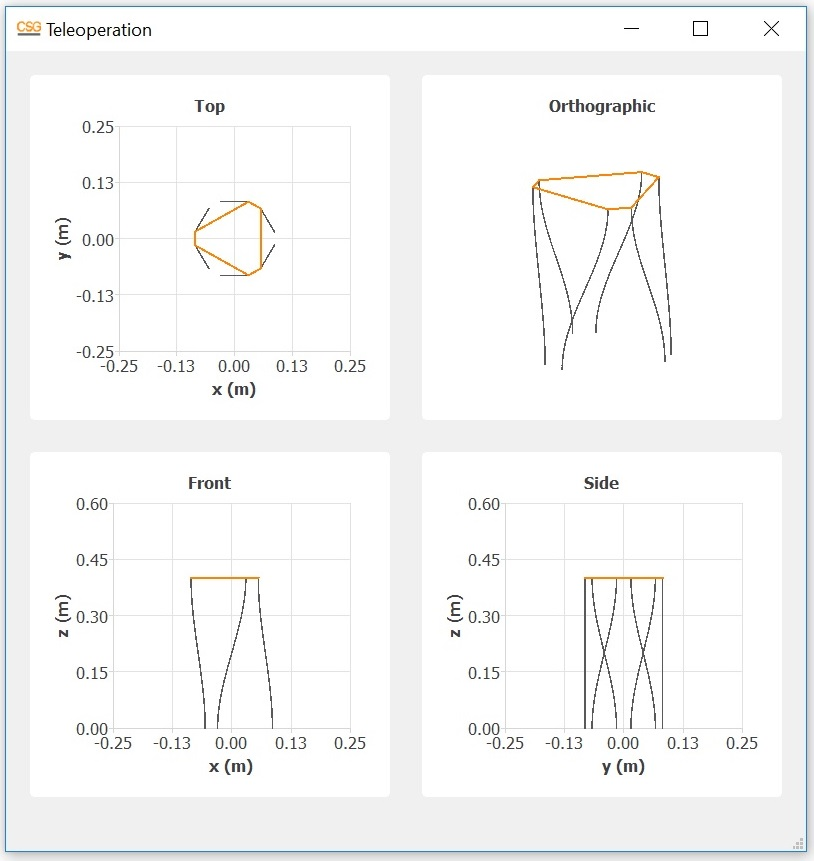
\includegraphics[width=0.46\textwidth]{fig/Home.jpg}
\end{figure}

\noindent
However, the program will not respond to user input yet.

\noindent To achieve keyboard input, we override the ``keyPressEvent'' function in the main window:
\begin{lstlisting}
void MainWindow::keyPressEvent(QKeyEvent* event){
    const double v_incr = 1e-4;
    const double w_incr = 1e-3;
    const int steps = 25;

    Vector3d vE = Vector3d::Zero();
    Vector3d wE = Vector3d::Zero();

    switch(event->key()){
        case !-\textcolor{QtPurpleColor}{Qt}-!::Key_A: vE.!-\textcolor{QtFunctionColor}{x}-!() -= v_incr; break;
        case !-\textcolor{QtPurpleColor}{Qt}-!::Key_D: vE.!-\textcolor{QtFunctionColor}{x}-!() += v_incr; break;
        case !-\textcolor{QtPurpleColor}{Qt}-!::Key_S: vE.!-\textcolor{QtFunctionColor}{y}-!() -= v_incr; break;
        case !-\textcolor{QtPurpleColor}{Qt}-!::Key_W: vE.!-\textcolor{QtFunctionColor}{y}-!() += v_incr; break;
        case !-\textcolor{QtPurpleColor}{Qt}-!::Key_Q: vE.!-\textcolor{QtFunctionColor}{z}-!() -= v_incr; break;
        case !-\textcolor{QtPurpleColor}{Qt}-!::Key_E: vE.!-\textcolor{QtFunctionColor}{z}-!() += v_incr; break;
        case !-\textcolor{QtPurpleColor}{Qt}-!::Key_I: wE.!-\textcolor{QtFunctionColor}{x}-!() -= w_incr; break;
        case !-\textcolor{QtPurpleColor}{Qt}-!::Key_K: wE.!-\textcolor{QtFunctionColor}{x}-!() += w_incr; break;
        case !-\textcolor{QtPurpleColor}{Qt}-!::Key_J: wE.!-\textcolor{QtFunctionColor}{y}-!() -= w_incr; break;
        case !-\textcolor{QtPurpleColor}{Qt}-!::Key_L: wE.!-\textcolor{QtFunctionColor}{y}-!() += w_incr; break;
        case !-\textcolor{QtPurpleColor}{Qt}-!::Key_U: wE.!-\textcolor{QtFunctionColor}{z}-!() -= w_incr; break;
        case !-\textcolor{QtPurpleColor}{Qt}-!::Key_O: wE.!-\textcolor{QtFunctionColor}{z}-!() += w_incr; break;
        case !-\textcolor{QtPurpleColor}{Qt}-!::!-\textcolor{QtPurpleColor}{Key\_Space}-!: resetKinematicsSolver();
    }

    try{
        for(int i = 0; i < steps; i++){
            pE += vE;
            RE += hat(wE)*RE;
            L = inverseKinematicsCSG(pE,RE);
        }
    }catch(...){
        resetKinematicsSolver();
    }
    refreshCharts();
}
\end{lstlisting}
Depending on which key is pressed, there is some velocity or angular velocity. We handle each different key press and then update the velocities based on the result. We use a loop to step through the kinematic solution, which is not strictly necessary, but hopefully will improve the solver robustness. Finally we update the charts based on the new configuration.

There is one problem. We are relying on convex optimization to solve the kinematics, and we may not find a minimum which meets the tolerance in a satisfactory number of iterations. If the solver ever fails to find a solution, we want to handle it gracefully. Although maybe not ideal, the most straightforward solution is to start over with the robot in the initial configuration, which we accomplish with another member function:
\begin{lstlisting}
void MainWindow::resetKinematicsSolver(){
    resetCSG();
    pE = 0.4*Vector3d::UnitZ();
    RE = Matrix3d::Identity();
    L = inverseKinematicsCSG(pE,RE);
}
\end{lstlisting}
In the first step, we need to reset the convex optimization guess so that we won't find ourselves in the same predicament the next time we invoke the solver. Then we solve the inverse kinematics to re-initialize the robot model. Resetting the guess is accomplished by a short function in the kinematics header:

\begin{lstlisting}
/*! Reset the convex optimization guess. */
inline void resetCSG(){
    guess << VectorXd::Zero(30), 0.4*VectorXd::Ones(6);
}
\end{lstlisting}

Now if we run the program, the robot will respond to keystrokes and move around. The teleoperation loop can even run fluidly on a Raspberry Pi 3B, so the kinematics solution speed is satisfactory. The core of a control scheme is in place; Qt has capabilities for serial communication if we wanted to extend this program to communicate with robotic hardware, but we won't worry about controlling the linear actuators on a physical robot here.
\begin{figure}[h]
	\centering
		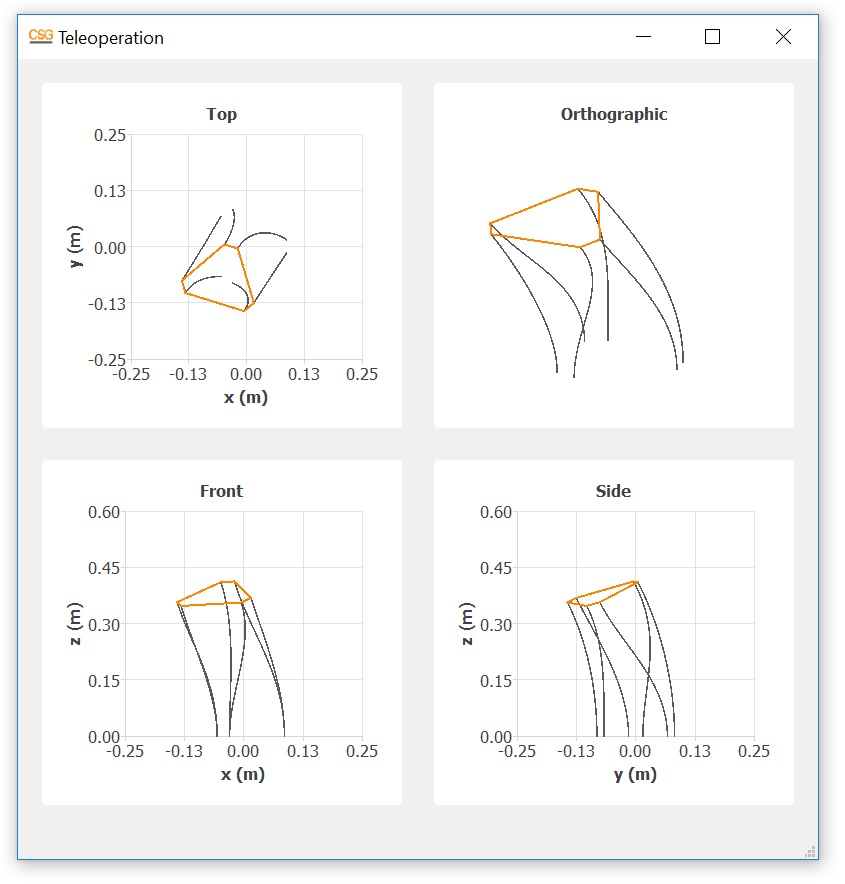
\includegraphics[width=0.9\textwidth]{fig/Moved.jpg}
\end{figure}

\end{document}